\label{chap:data}
Um Daten von übermüdeten Fahrern zu erhalten, kann natürlich kein Versuch im Straßenverkehr durchgeführt werden. Die Fremd- und Eigengefährdung ist zu groß. Darum finden die Versuche in der Simulationsumgebung der \acl{RTU} statt. Für das Experiment wird im Fahrsimulator eine Nacht-Autobahnfahrt simuliert. Verschiedene Studien \cite{Engstrom_2322937}, \cite{Horne_1757738} legen nahe, dass sich Simulationen zwar von der Realität unterscheiden, dass  die Ergebnisse jedoch trotzdem valide und brauchbar sind.

Für den Versuch werden neben den rohen EEG Signalen, auch die Fahrzeugdaten, sowie ein Video der Simulation und des Fahrers aufgenommen. Weiterhin kann der Versuchsleiter Besonderheiten protokollieren (Abb. \ref{fig:experiment}).

\begin{figure}[h] 
  \begin{center}
    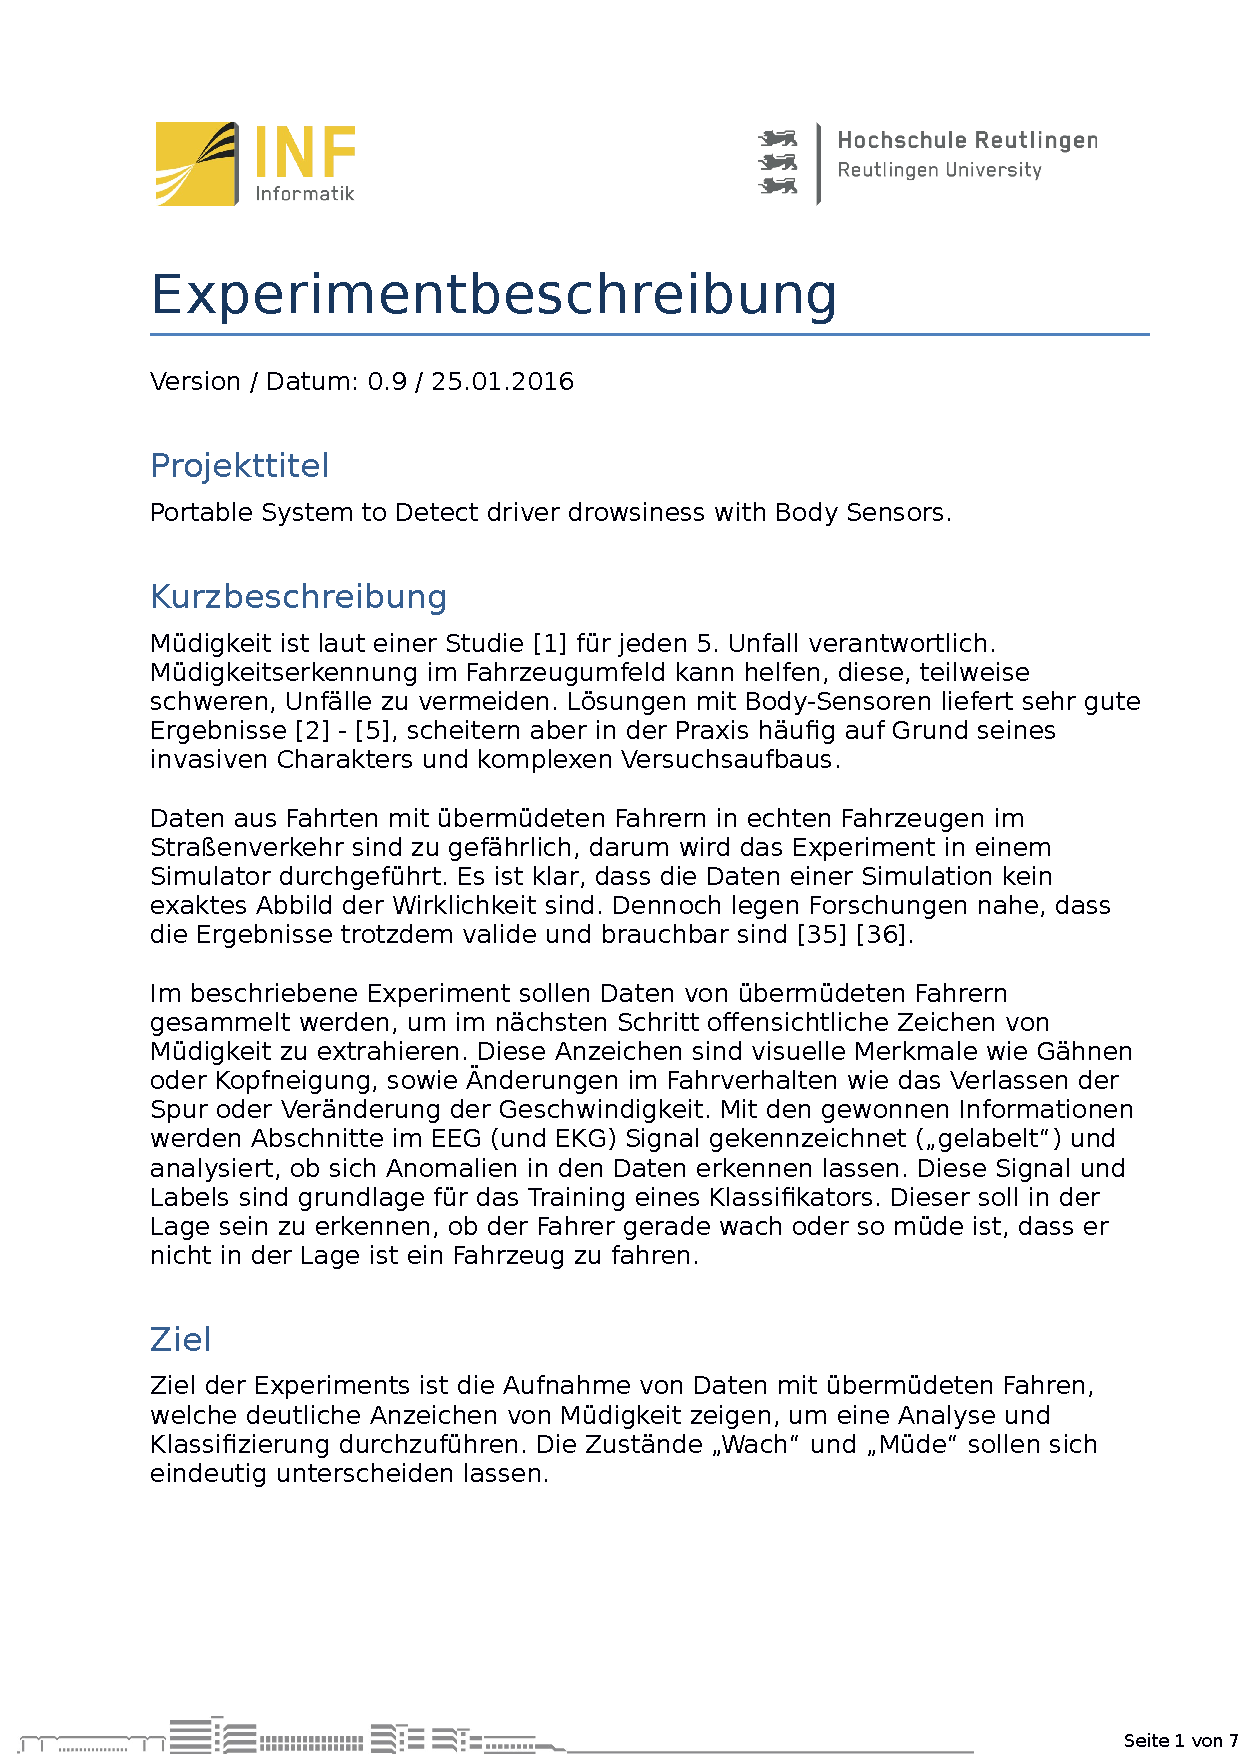
\includegraphics[width=\columnwidth]{experiment}
    \caption[Versuchsaufbau Experiment]{Der Versuchsaufbau für die Erkennung von Müdigkeit mit den Datenströmen aus der Fahrerkabine zur Testüberwachung. \label{fig:experiment}}
  \end{center}
\end{figure}

Im Versuch sollte der Fahrer, mit fortschreiten des Versuchs, immer mehr eindeutige Anzeichen von Müdigkeit zeigen. Dies kann durch verschiedene Versuchsparameter begünstigt werden. So zeigt eine Studie, dass Unfälle meist zwischen 2:00 - 6:00, sowie 14:00 - 16:00 Uhr passieren \cite{Horne_1757738}. Auch die Schlafmenge von weniger als 6 Stunden in der Nacht vor dem Experiment erhöht die Chance auf Anzeichen \cite{Engstrom_2322937}. Das Geschlecht oder Alter der Probanden ist nicht relevant. Vor dem Experiment sollten jedoch keine Drogen, Alkohol oder Kaffee eingenommen werden. Ein Führerschein ist von Vorteil, aber nicht zwingend notwendig.

Auch die Teststrecke (Abb. \ref{fig:drivingtask}) trägt zur Erhöhung der Müdigkeit bei. Monotone Autobahnfahrten die größtenteils geradeaus verlaufen, ohne andere Verkehrsteilnehmer und konstanter Geschwindigkeit führen eher zu einer Ermüdung. Nach diesen Kriterien wurde eine endlose zweispurige Autobahnkarte mit einer Geschwindigkeit von konstant 130Kmh erstellt. Sie spielt zudem Nachts und ist somit dunkel gehalten, was besonders anstrengend für die Augen ist. Die Simulation ist auf Bildschirm vermutlich noch anstrengender als eine echte Aussicht durch ein Autofenster.

\begin{figure}[h] 
  \begin{center}
    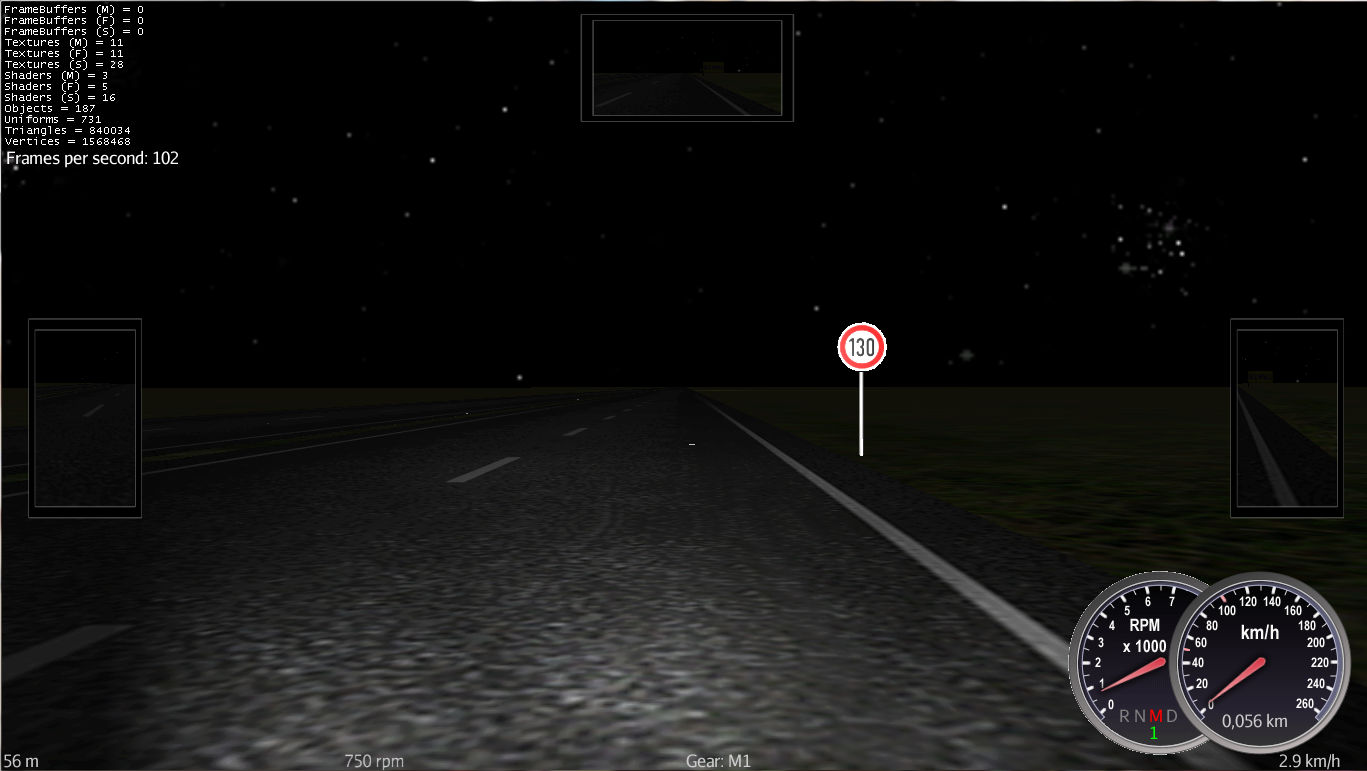
\includegraphics[width=0.75\columnwidth]{drivingtask}
    \caption[Driving Task Screenshot]{Die Autobahnkarte für den Versuch verläuft endlos geradeaus und spielt nachts bei konstanter Geschwindigkeit. \label{fig:drivingtask}}
  \end{center}
\end{figure}

Für einen Versuch werden 40 Minuten angesetzt. Fünf Minuten werden für eine kurze Einführung und Einrichten des EEGs, 30 Minuten für die Testfahrt und wieder fünf Minuten für eine kurze Selbsteinschätzung mit Fragebogen.

Anhand der aufgenommenen Daten werden nun Stellen gesucht, an denen die Testperson eindeutige Anzeichen von Müdigkeit zeigt. Eindeutig sind Verhaltensweisen wie häufiges Gähnen und Einnicken (Kopf fällt nach vorn) - diese Merkmale werden häufig in CV-Ansätzen genutzt. 
Auch Verhaltensmerkmale wie, von der Spur abkommen und heftig Gegenlenken oder deutliche Veränderungen der Geschwindigkeit können Anzeichen für eine Unachtsamkeit aufgrund von Müdigkeit sein. Diese Stellen werden dann in den EEG Daten mit dem Label "`Müde"' markiert, alle anderen mit "`Wach"'. Die EEG Sequenzen können dann auf eindeutige Varianzen untersucht werden. 

Das Experiment wurde mit 4 Personen (m / w) durchgeführt. Das Einrichten des EEG-Headsets (alle Sensoren auf hoher Qualität) war aufwändiger als erwartet, klappte jedoch bei allen Personen. Aus organisatorischen Gründen, fand nur ein Teil der Experimente nachmittags statt, der Rest fuhr morgens. Die Teilnehmer hatte im Vorfeld verschieden lang geschlafen und bewerteten auch die jeweilige Schlafqualität unterschiedlich. Die Testpersonen gaben an, vor dem Experiment eher wach als müde zu sein. Alle Fahrer gaben an, schon einmal übermüdet gefahren zu sein, waren sich aber nicht einig, ob sie sich eine Müdigkeitserkennung in einen Neuwagen bestellen würden.

Nach der Testfahrt gaben alle Teilnehmer an, müder als vorher gewesen zu sein. Dies zeigt sich auch an visuellen Merkmalen in den letzten Minuten der Testfahrt. Wobei die Ausprägungen der einzelnen Fahrer durchaus unterschiedlich war. Visuelle Anzeichen von Müdigkeit waren den Testpersonen bekannt (Gähnen, häufige Positionswechsel, häufiges Blinzeln, trockene Augen) und konnten diese an sich selbst beobachten. Auch die Fahrweise zeigte teilweise deutliche Anzeichen von Unkonzentriertheit (Abkommen von der Spur, Schlangenlinien, zu niedrige / hohe Geschwindigkeit)\drivingTask


Die Eigen- und Außenwahrnehmung bestätigt die Hypothese, dass es während des Experiments zu einem Abfall der Wachheit kommt und sich dies an Hand der erwarteten Merkmale zeigte. Die Veränderungen der Aufmerksamkeit muss nun im EEG Signal extrahiert werden.